% - - - - - - - - - -
% Packages and document configuration
% - - - - - - - - - -

\documentclass[paper=a4, fontsize=11pt]{scrartcl} % A4 paper and 11pt font size

\usepackage[T1]{fontenc} % Use 8-bit encoding that has 256 glyphs
\usepackage{fourier} % Use the Adobe Utopia font for the document - comment this line to return to the LaTeX default
\usepackage[english]{babel} % English language/hyphenation
\usepackage{amsmath,amsfonts,amsthm} % Math packages

\usepackage{lipsum} % Used for inserting dummy 'Lorem ipsum' text into the template

\usepackage{sectsty} % Allows customizing section commands
%\allsectionsfont{\centering \normalfont\scshape} % Make all sections centered, the default font and small caps

\usepackage{fancyhdr} % Custom headers and footers
\pagestyle{fancyplain} % Makes all pages in the document conform to the custom headers and footers
\fancyhead{} % No page header - if you want one, create it in the same way as the footers below
\fancyfoot[L]{} % Empty left footer
\fancyfoot[C]{} % Empty center footer
\fancyfoot[R]{\thepage} % Page numbering for right footer
\renewcommand{\headrulewidth}{0pt} % Remove header underlines
\renewcommand{\footrulewidth}{0pt} % Remove footer underlines
\setlength{\headheight}{13.6pt} % Customize the height of the header

%\numberwithin{equation}{section} % Number equations within sections (i.e. 1.1, 1.2, 2.1, 2.2 instead of 1, 2, 3, 4)
%\numberwithin{figure}{section} % Number figures within sections (i.e. 1.1, 1.2, 2.1, 2.2 instead of 1, 2, 3, 4)
%\numberwithin{table}{section} % Number tables within sections (i.e. 1.1, 1.2, 2.1, 2.2 instead of 1, 2, 3, 4)

\setlength\parindent{0pt} % Removes all indentation from paragraphs - comment this line for an assignment with lots of text

\usepackage{graphicx}
\usepackage{xcolor}

% - - - - - - - - - -
% Title
% - - - - - - - - - -

\newcommand{\horrule}[1]{\rule{\linewidth}{#1}} % Create horizontal rule command with 1 argument of height

\title{
	\normalfont \normalsize 
	\textsc{School of Informatics, University of Edinburgh} \\ [25pt] % Your university, school and/or department name(s)
	\horrule{0.5pt} \\[0.4cm] % Thin top horizontal rule
	\huge Informatics Large Practical Coursework 1 \\ % The assignment title
	\horrule{2pt} \\[0.5cm] % Thick bottom horizontal rule
}

\author{CHENG LI \\ s1603732}
\date{11/10/2018}

\begin{document}
\maketitle

% - - - - - - - - - -
% Part one
% - - - - - - - - - -
\section{Introduction}
\paragraph{} This project plan includes the basic structure of my Coinz game, together with the fundamental settings and bonus features. The rationale for using Kotlin as the programming language for this application is also included. Moreover, there is a week-by-week schedule for implementation.

% - - - - - - - - - -
% Part two
% - - - - - - - - - -
\section{Design Decisions}
\subsection{Diagram}
\begin{figure}
	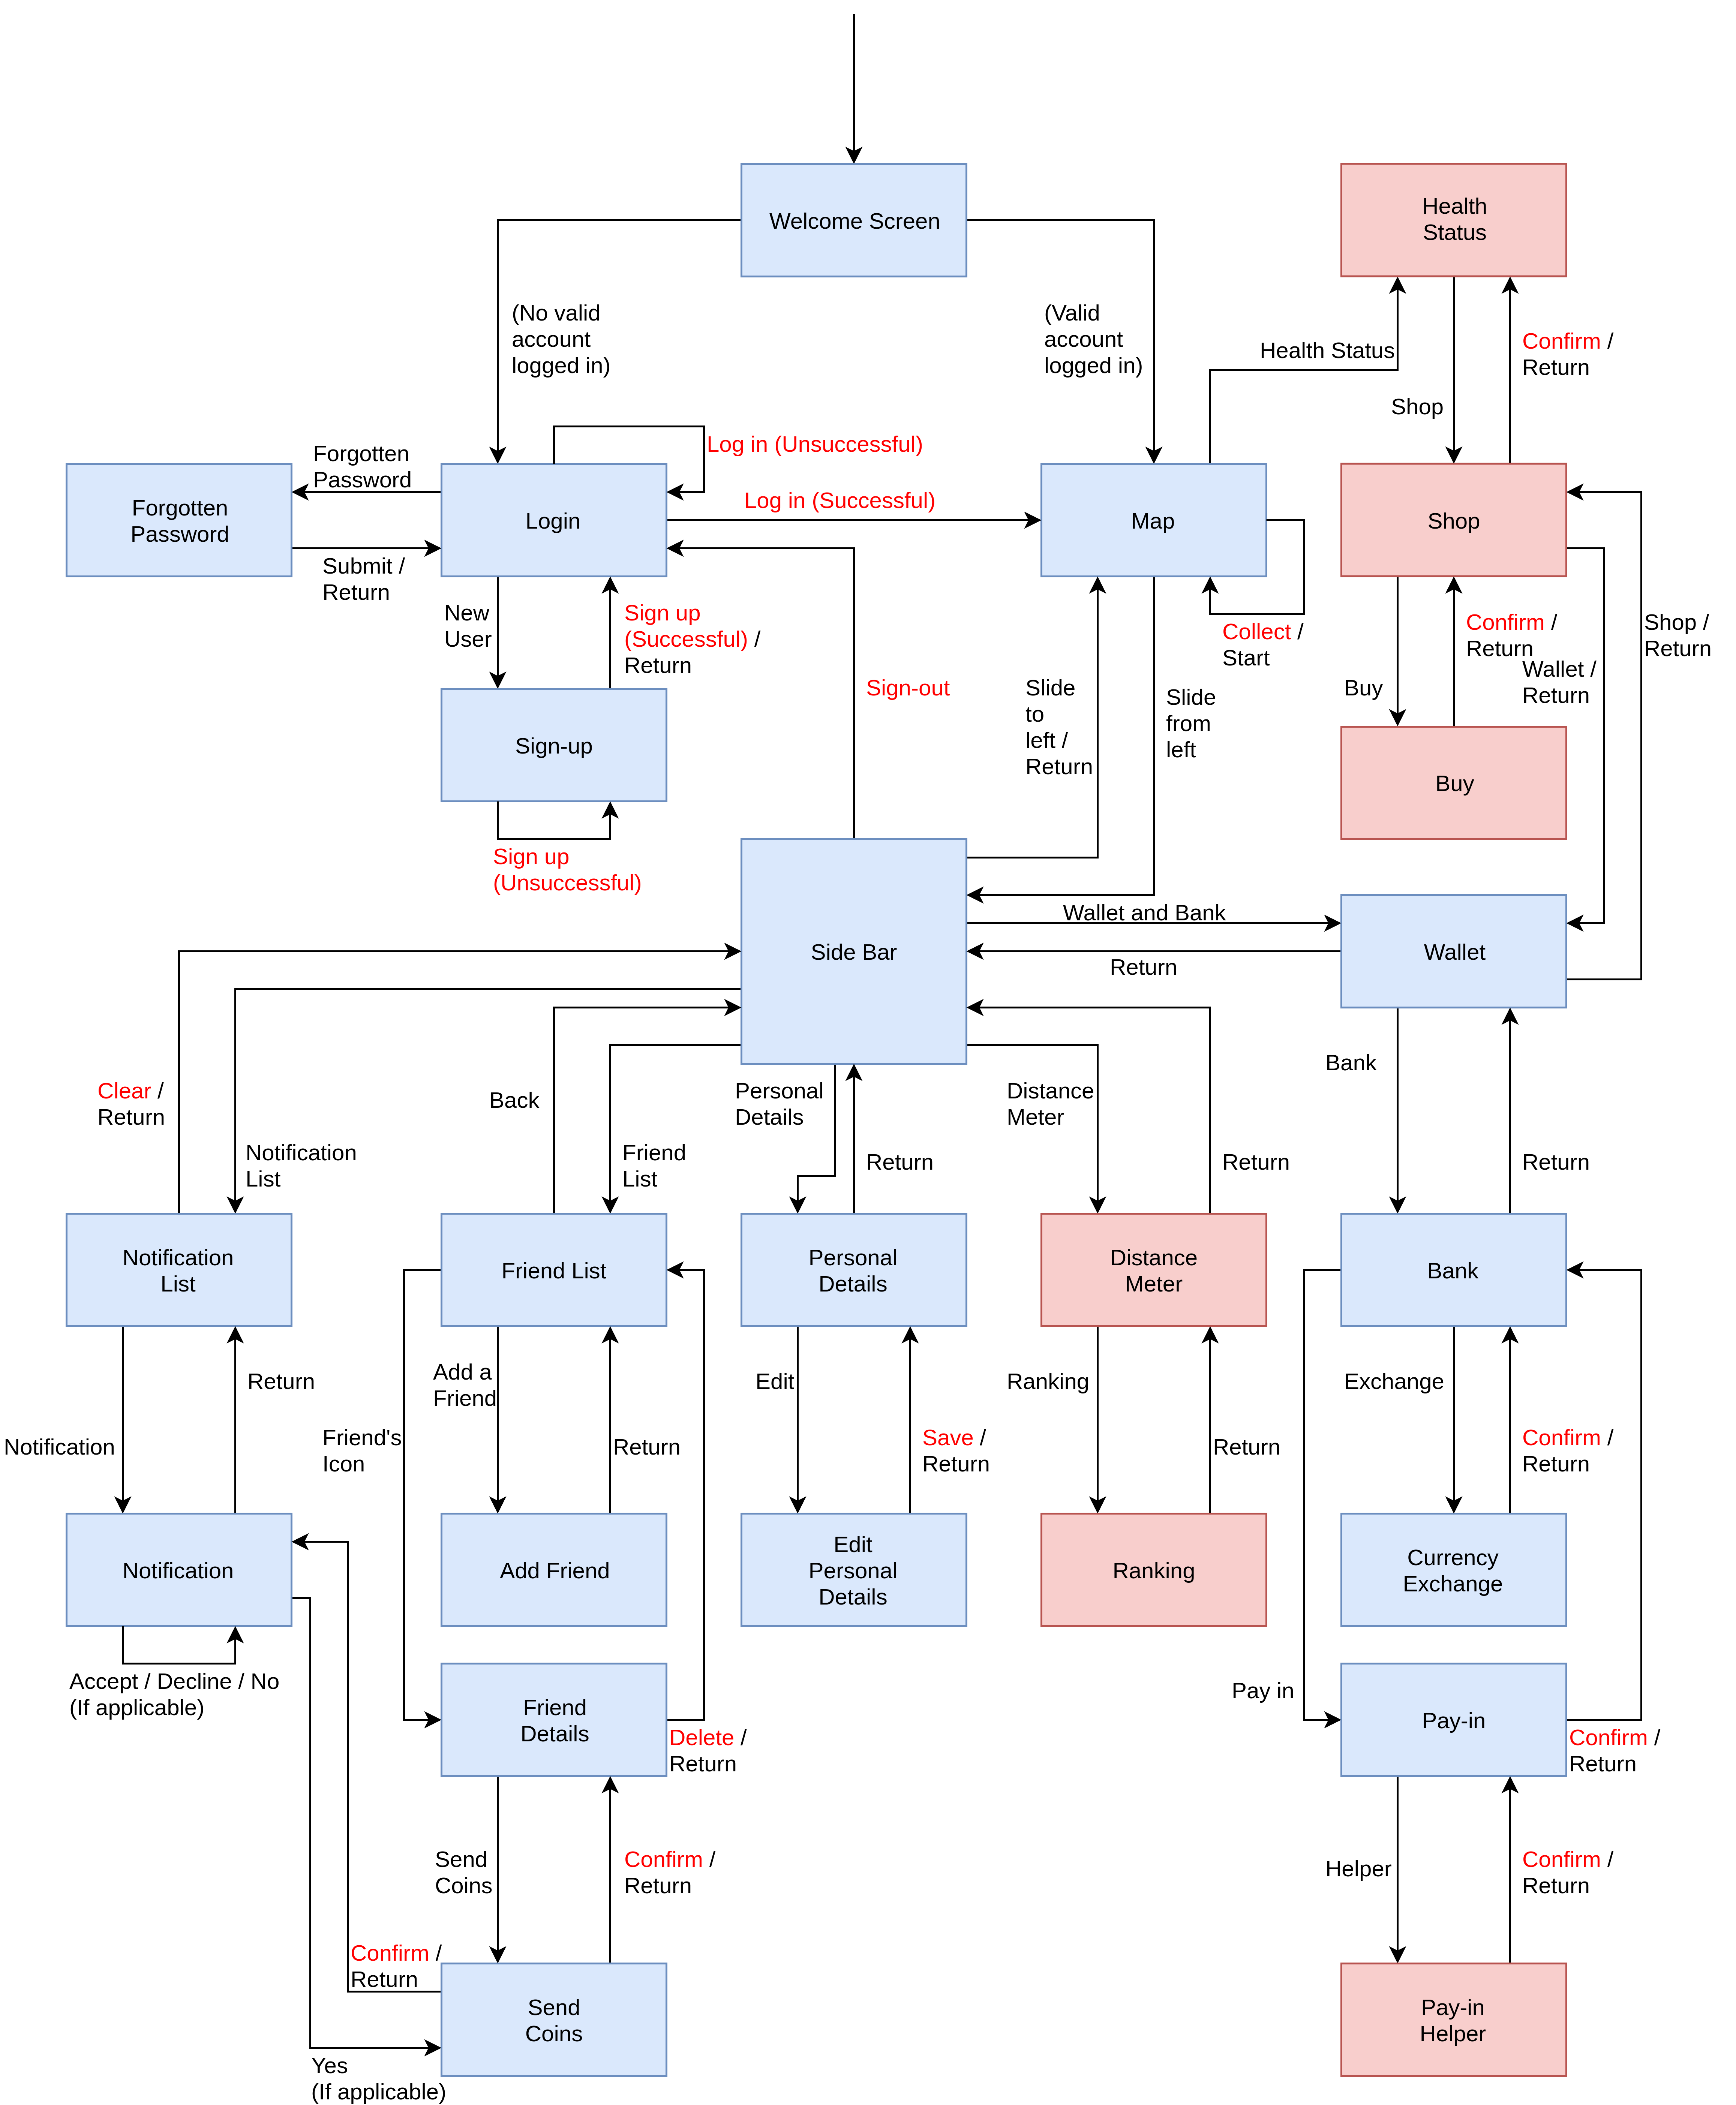
\includegraphics[width=\linewidth]{Coinz.png}
	\caption{Activities}
	%\label{fig:boat1}
\end{figure}
%Figure \ref{fig:boat1} shows a boat.
\paragraph{} $\bullet$ Diagram is shown as Figure 1.
\paragraph{} $\bullet$ Basic features are in blue rectangles, while bonus features are in red rectangles.
\paragraph{} $\bullet$ Words (without brackets) near the arrow indicates the name of the buttons used for switching activities.
\paragraph{} $\bullet$ Pop-up windows would show up after clicking the buttons of which the words are in red. For example, after clicking the "\textcolor{red}{Confirm}" button, a pop-up window with text "Are you sure you want to do <something> ?" and two buttons reads "Yes" and "No" respectively would come up. 
\paragraph{} $\bullet$ Slashes indicates multiple buttons.
\paragraph{} $\bullet$ "Return" button indicates the return button from the Android System.
\paragraph{} $\bullet$ Words with brackets indicates the system status at certain stage.


\subsection{Activities}
\paragraph{}$\bullet$ \textbf{Welcome Screen: } If the game does not have a valid account logged in, it will lead to the "Login" page. Otherwise, the "Map" page would show up at this stage.
\paragraph{}$\bullet$ \textbf{Login: } This page contains a "sign-up" button for new users to the game, a "sign-in" button for users with a valid account and a "forgotten password" button for users who have forgotten their password.
\paragraph{}$\bullet$ \textbf{Sign-up: } This page contains several blanks used for filling in the users basic informations such as first name, surname, nickname, gender, email address and password. If the email addressed has been used, password is too short or names are too long, the sign-up would be unsuccessful, otherwise clicking the "Sign up" button would create an account and come back to "Login" page.
\paragraph{}$\bullet$ \textbf{Forgotten Password: } This page contains a blank for entering the email address. After clicking the "Submit" button, the user would receive an email with one's new password, which could be changed later, in it if the account does exist and the "Login" page would show up. 
\paragraph{}$\bullet$ \textbf{Map: } This page contains a map as the playground of this game, with coins marked and scattered in it. Also, a "Side Bar" is hidden on the left of the screen and a "Health Status" button on the top right corner.
\paragraph{}$\bullet$ \textbf{Side Bar: } This page contains multiple buttons used for accessing other pages provided in the game.
\paragraph{}$\bullet$ \textbf{Personal Details: } This page list out the basic information of the current user, together with a "Edit" button used for editing the details.
\paragraph{}$\bullet$ \textbf{Edit Personal Details: } This page list out the basic information of the current user, and each line would have a blank used for entering the new information the user would like to change. Also, a "Save" button is provided to update the new information. However, the button would be disabled if the new password is too short or the new names are too long.
\paragraph{}$\bullet$ \textbf{Wallet: } This page contains the current balance for the four kinds of currencies and their corresponding and total "Gold Coin" value with the current rate. Also, a "Bank" button is provided to enter the bank and make transactions, and a "Shop" button is provided to enter the shop and buy things. Spare coins would expire at the end of the day.
\paragraph{}$\bullet$ \textbf{Bank: } This page contains the balance for the five kinds of currencies in the bank, together with the current rate for each of the four currencies to "Gold Coin" and the other way round. Also, there are four "Exchange" buttons for the four currencies, all leads to the "Currency Exchange" page and one "Pay in" button for paying coins from the wallet into the bank account.
\paragraph{}$\bullet$ \textbf{Currency Exchange: } This page contains the current rate for the specific currency you want to exchange, options for the direction of exchange and a blank for  entering the expected amount.
\paragraph{}$\bullet$ \textbf{Pay in: } This page allows you to choose 25 coins to pay into the account.
\paragraph{}$\bullet$ \textbf{Friend List: } This page lists all the friends you currently have. Also, an "Add a friend" button is available for adding new friends, an "Delete" button is available for deleting a friend and clicking the icon of the friend would lead to his "Friend Details" page.
\paragraph{}$\bullet$ \textbf{Friend Details: } This page shows the basic information of a friend. Also, a "Send Coins" button could be used to send coins to this friend.
\paragraph{}$\bullet$ \textbf{Send Coins: } This page allows user to send spare coins to a friend.
\paragraph{}$\bullet$ \textbf{Notification List: } This page shows the notifications received and by clicking a line of notification, the detailed notification would show up.
\paragraph{}$\bullet$ \textbf{Notification: } This page shows the full text of the notification. If this notification is about adding new friends, the "Accept" and "Decline" buttons are used for accepting the invitation or not. If this notification is about receiving coins from a friend, the "Yes" and "No" buttons are used for decision on whether sending coins back to the friend or not. If the "Yes" button is pressed, "Send Coins" page would come up.



\subsection{Bonus Features}
\subsubsection{Health Status}
\paragraph{} The health status in the world of this game is defined as: Every "playing" day (user starts the game at least once that day), users need enough bread, meat and water or pills to maintain vitality during the game. Bread, meat and water could be purchased in the store by using "SHIL", "DOLR", "QUID" and "PENY" respectively. When a new maps come out, users have a 10-minute window to collect enough coins for buying bread, meat and water. After 10 minutes, the coins would temporarily disappear on the map until enough bread, meat and water is purchased, but the shop is still accessible. If a user fails to obtain enough bread, meat and water but has pills left in the bag, the user could consume a pill and have another 10-minute window. How many pills a user could consume daily is not limited, as long as there are pills left in the bag and the bag could only contains at most 5 pills all the time. Moreover, a friend could not help you (sending coins to you) at this stage.
\paragraph{}$\bullet$ \textbf{Health Status: } This page contains the current balance and the capacity of bread, meat, water and pills. Also, a "Shop" button could be used to access the shop directly.
\paragraph{}$\bullet$ \textbf{Shop: } This page contains the prices of the essentials and the "Buy" button for making a purchase. Also, the "Wallet" page could be accessed from here.
\paragraph{}$\bullet$ \textbf{Buy: } This page contains the details for buying a certain kind of thing.

\subsubsection{Play Against Time}
\paragraph{} As mentioned previously, the start of the game is a 10-minute window which allows the user to collect enough coins for buying the essentials. And a new 10-minute window will show up when a user consumes a pill.

\subsubsection{Distance Meter}
\paragraph{}$\bullet$ \textbf{Distance Meter: } This page shows the distance user has covered during the game till now. Also, a "Ranking" button is provided to see the ranking.
\paragraph{}$\bullet$ \textbf{Ranking: } This page shows the ranking of distance covered among friends.

\subsubsection{Paid Helper}
\paragraph{}$\bullet$ \textbf{Pay-in Helper: } This page contains a paid service which could help the user find out the first 26 most valuable coins at a cost of the most valuable coin (the most valuable coin is used to pay for this service and the rest 25 coins would be paid into the bank; value is based on the current rate). Users with less than 26 coins are not eligible for this service.





%\paragraph{}$\bullet$ \textbf{Level and Medal: } Users could earn experience by collecting points and experience could be used for levelling up. Users could also participating in activities and events to get corresponding medals and limited events would have limited medals.
%\paragraph{}$\bullet$ \textbf{Cash Back: } Monthly, the user with the most money could get cash back.

%\paragraph{}$\bullet$ \textbf{Advertisement and Membership: } As the game would be a free game, so the profit would come from advertisement. Users would see a pop-up advertising each time they enter the game, and simply by clicking the right corner cross, the advertisement would disappear. For better services, people could buy membership in order to stop the notification of advertisement. At this stage, membership could only be purchased by the coin collected in the game.
%\paragraph{}$\bullet$ \textbf{Personalisation: } This feature is exclusive to members only. Members could personalise their theme for the game.


% - - - - - - - - - -
% Part three
% - - - - - - - - - -
\section{Development Language - Kotlin}
\subsection{Conciseness}
\paragraph{} The syntax of Kotlin is much more concise and intuitive compared to Java which would make the team more productive, since the same code could be written in fewer lines.
\subsection{Null Safety}
\paragraph{} Compared to Java, Kotlin is safer when dealing with null, since situations with null are handled during compiling, which would help avoid the abnormality during execution. If an object could be null, we need to clearly assign it and to check whether it is null during usage. Time would be saved, because no more "NullPointerExceptions".
\subsection{Fully Supported}
\paragraph{} In 2017, Google announced that Kotlin is the officially supported language in Android. Also, both Kotlin and Android Studio are developed by the same company JetBrains. Both reliability and convenience are without doubt.
\subsection{Interoperability with Java}
\paragraph{} Java codes and libraries could be used in a Kotlin project because of the wonderful interoperability. Also, it is not hard to learn Kotlin from scratch for a team member since they are quite alike.
\subsection{Extension Functions}
\paragraph{} We could extend classes with more features even if we do not have the access to the source code.
\subsection{Functional Programming Support}
\paragraph{} Brilliant support for features from a functional programming language.
\subsection{Better API Designs}
\paragraph{} Due to inherent limitations, using Java would experience some problems with Android API design, while using Kotlin would experience much less problems.
\subsection{String Interpolation}
\paragraph{} Building strings would be more satisfying.

% - - - - - - - - - -
% Part four
% - - - - - - - - - -
\section{Week-by-week Timetable}
\subsection{Week 1}
\paragraph{}$\bullet$ Preparations for the start of the semester.
\subsection{Week 2}
\paragraph{}$\bullet$ Get familiar with Android developing.
\subsection{Week 3}
\paragraph{}$\bullet$ Get familiar with Android developing
\paragraph{}$\bullet$ Get familiar with version controls.
\subsection{Week 4}
\paragraph{}$\bullet$ Finish coursework 1.
\subsection{Week 5}
\paragraph{}$\bullet$ Map interface fully implemented:
\subparagraph{}\quad $\ast$ Location of coins refreshes daily.
\subparagraph{}\quad $\ast$ Coins could be picked up when user is within 25 meters.
\paragraph{}$\bullet$ Side bar interface partly implemented.
\subsection{Week 6}
\paragraph{}$\bullet$ Viewing and editing personal details and linkage with side bar fully implemented.
\paragraph{}$\bullet$ Login system fully implemented:
\subparagraph{}\quad $\ast$ Sign-in, sign-up and forgotten password all work fine.
\subparagraph{}\quad $\ast$ User should receive an email when signing in or retrieving password.
\paragraph{}$\bullet$ Welcome screen fully implemented.
\subsection{Week 7}
\paragraph{}$\bullet$ Friend list and notification list fully implemented:
\subparagraph{}\quad $\ast$ Users could add friends and also could be added as a friend by others.
\subparagraph{}\quad $\ast$ Users could receive coins from and send coins to their friends.
Implement the banking system.
\subsection{Week 8}
\paragraph{}$\bullet$ Wallet interface fully implemented.
\paragraph{}$\bullet$ Banking system fully implemented:
\subparagraph{}\quad $\ast$ Users could make currency exchanges.
\subparagraph{}\quad $\ast$ Users could pay in with five kinds of currencies.
\subparagraph{}\quad $\ast$ Eligible users could pay to use the helper service.
\subsection{Week 9}
\paragraph{}$\bullet$ Health status system fully implemented:
\subparagraph{}\quad $\ast$ Works fine as the description given previously.
\paragraph{}$\bullet$ Timing system fully implemented.
\subsection{Week 10}
\paragraph{}$\bullet$ Distance meter fully implemented.
\paragraph{}$\bullet$ Ranking fully implemented.
\subsection{Week 11}
\paragraph{}$\bullet$ Necessary linkages fully implemented.
\paragraph{}$\bullet$ Testing and debugging.
\subsection{Week 12}
\paragraph{}$\bullet$ Testing and debugging.
\subsection{Week 13}
\paragraph{}$\bullet$ Testing and debugging.
\paragraph{}$\bullet$ Submission.

\end{document}
